 \documentclass[11pt]{beamer}
 \usetheme{Madrid}
 \usepackage[utf8]{inputenc}
 \usepackage[french]{babel}
 \usepackage[T1]{fontenc}
 \usepackage{amsmath}
 \usepackage{amsfonts}
 \usepackage{amssymb}
 \usepackage{graphicx}
 \usepackage{algorithm2e}
 \author{\textbf{Présenté par:} \\ \textit{Tafsir GNA} \\ \textbf{Supervisé par:} \\ \textit{Dr Ing. Vinasétan Ratheil HOUNDJI \\ \& \\ Professeur Mahouton Norbert HOUNKONNOU}}
 \title{Résolution du \emph{Pigment Sequencing Problem} avec les algorithmes génétiques}
 %\setbeamercovered{transparent} 
 %\setbeamertemplate{navigation symbols}{} 
 %\logo{} 
\institute{Institut de Formation et de Recherche en Informatique (IFRI)} 
 %\date{} 
 %\subject{} 
 \begin{document}
 
 \begin{frame}
	\hbox to \textwidth
 	{
 		
\includegraphics[scale=0.2]{img/ifri_logo.png}
 		\hfill
 		\texttt{Mémoire de master en Informatique}
 		\hfill
 		
\includegraphics[scale=0.2]{img/uac_logo.png}
 	}
	\titlepage
\end{frame} 


 
 % Page de sommaire
 \begin{frame}
 \frametitle{Sommaire}
 \tableofcontents
 \end{frame}
 
 % Introduction
 \section*{Introduction}
 \begin{frame}
 \frametitle{Introduction}
 	\begin{center}
 		\LARGE{\texttt{Introduction}}
 	\end{center}
 \end{frame}
 
 % Etat de l'art
 \section{Etat de l'art}
 \subsection{Le dimensionnement de lots en planification de production}
 \begin{frame}
 \frametitle{Le dimensionnement de lots en planification de production}
 \framesubtitle{Critères de classification}
 	%Différents critères [] interviennent dans la classification des problèmes de dimensionnement de lots, notamment :
	\begin{itemize}
		\item L’échelle de temps;
		\item Le nombre de niveaux;
		\item Le nombre de produit;
		\item Les contraintes de capacité;
		\item Les demandes;
		\item Les coûts et temps de lancement ou préparation (setup).
	\end{itemize}
 \end{frame}
 
 \begin{frame}
 \frametitle{Le dimensionnement de lots en planification de production}
 \framesubtitle{Classes de problèmes de dimensionnement de lots I}
 	%Suivant l’échelle en temps, nous distinguons les classes de problèmes de dimensionnement de lots comme suit:
	\begin{itemize}
		\item Problèmes de petite taille ou à courtes périodes;
		\item Problèmes de grande taille ou à longues périodes;
		\item Problèmes de très grande taille ou à très longues périodes.
	\end{itemize}
 \end{frame}
 
 \begin{frame}
 \frametitle{Le dimensionnement de lots en planification de production}
 \framesubtitle{Classes de problèmes de dimensionnement de lots II}
 	%Nous nous sommes intéressés au cours de notre travail aux problèmes de petite taille ou à courtes périodes au sein desquels nous pouvons distinguer:
	\begin{itemize}
		\item Discrete lot-sizing and scheduling problem (DLSP);
		\item Continuous setup lot-sizing problem (CSLP);
		\item Proportional lot-sizing and scheduling problem (PLSP);
		\item General lot-sizing and scheduling problem (GLSP).
	\end{itemize}
	%Le "Pigment Sequencing Problem" fait partie de la famille DLSP.
 \end{frame}
 
 \begin{frame}
 \frametitle{Le dimensionnement de lots en planification de production}
 \framesubtitle{Classes de problèmes de dimensionnement de lots III}
 \begin{center}
		\begin{figure}[!h]
			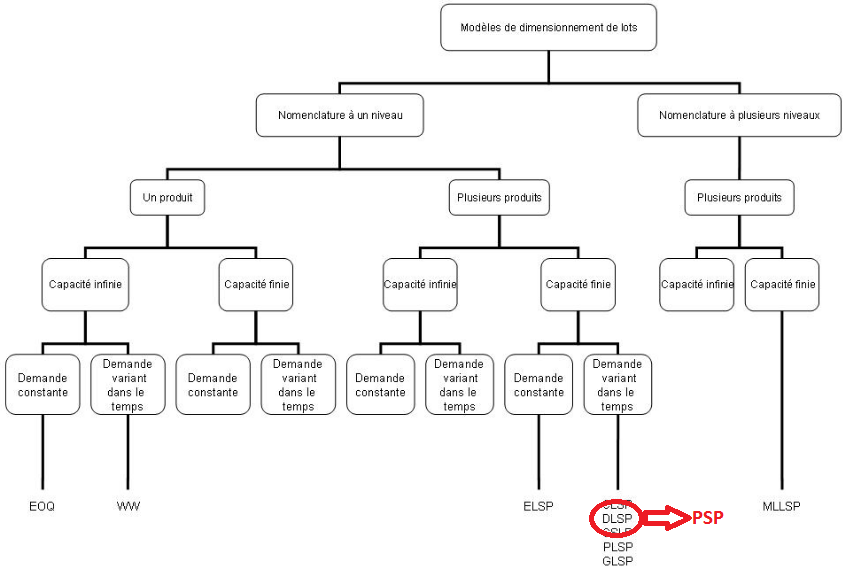
\includegraphics[scale=.3]{img/classification_dimensionnement.png}
			\caption{Exemple de classification des modèles de dimensionnement de lots []}
			\label{fig:classification_dimensionnement_lots}
		\end{figure}
	\end{center}
 \end{frame}
 
 \subsection{Le "Pigment Sequencing Problem" (PSP)}
 \begin{frame}
 \frametitle{Le "Pigment Sequencing Problem" (PSP)}
 \framesubtitle{Description}
 
 	Objectif:
    \begin{itemize}
    	\item trouver un plan de production de plusieurs articles à partir d’une
machine avec des coûts de transition;
    	\item respectant la capacité de production de la machine ;
    	\item minimisant les coûts de stockage et de transition.
    \end{itemize}
 \end{frame}
 
 \begin{frame}
 \frametitle{Le "Pigment Sequencing Problem" (PSP)}
 \framesubtitle{Modèles et formulations}
 
    \begin{itemize}
    	\item Modèles basés sur la programmation en nombres mixtes[] (MIP1, MIP2, MIP3);
    	\item Modèle basé sur la Programmation par contraintes[];
    	\item Modèle basé sur le recuit simulé[].
    \end{itemize}
 
 \end{frame}
 
 \subsection{Les algorithmes génétiques}
 \begin{frame}
 \frametitle{Les algorithmes génétiques}
 \framesubtitle{Algorithme génétique standard}
 
 	\begin{algorithm}[H]
 	\caption{Algorithme génétique standard \cite{Goncalves}}
 	\label{algo:algo_genetique_standard}
 	%\KwData{this text}
 	%\KwResult{how to write algorithm with \LaTeX2e }
 	%initialization\;
 	Générer la population initiale $P_{i}$ \\
 	Évaluer la population $P_{i}$ \\
 	\While{le critère de terminaison n'est pas satisfait}{
 	 Sélectionner les éléments de $P_{i}$ à copier dans $P_{i+1}$ \\
 	 Appliquer le croisement aux éléments de $P_{i}$ et les mettre dans $P_{i+1}$ \\
 	 Appliquer la mutation aux éléments de $P_{i}$ et les mettre dans $P_{i+1}$ \\
 	 Évaluer la nouvelle population $P_{i+1}$ \\
 	 $P_{i}$ = $P_{i+1}$
 	}
	\end{algorithm}
 \end{frame}
 
 
 \begin{frame}
 \frametitle{Les algorithmes génétiques}
 \framesubtitle{Opérations génétiques}
 
 	\begin{itemize}
 		\item la sélection;
 		\item le croisement;
 		\item la mutation.
 	\end{itemize}
 \end{frame}
 
 \begin{frame}
 \frametitle{Les algorithmes génétiques}
 \framesubtitle{Les algorithmes génétiques parallèles}
 
 	\begin{itemize}
 		\item Les algorithmes génétiques parallèles de type master-slave;
 		\item Les algorithmes génétiques parallèles coarse-grained;
 		\item Les algorithmes génétiques parallèles fine-grained.
 	\end{itemize}
 \end{frame}
 
 \begin{frame}
 \frametitle{Les algorithmes génétiques}
 \framesubtitle{Hiérarchisation entre les algorithmes génétiques parallèles}
 
 	\begin{itemize}
 		\item Les algorithmes génétiques parallèles et hiérarchiques entre coarse-grained et master-slave;
 		\item Les algorithmes génétiques parallèles et hiérarchiques entre coarse-grained et fine-grained.
 	\end{itemize}
 \end{frame}
 
 % Matériel et Méthodes
 \section{Matériel et Méthodes}
 \subsection{Outils de test}
 \begin{frame}
 \frametitle{Outils de test}
 %\framesubtitle{}
 
 	\begin{itemize}
 		\item Système d'exploitation: Linux Ubuntu 16.04 LTS; 
		\item Processeur: Intel®  Core \up{\textsc{TM}} i7 CPU L 640 @ 2.13GHz x 4; 
		\item Mémoire: 3,7 Gio;
		\item Type du système d'exploitation: 64 bits.
 	\end{itemize}
 \end{frame}
 
 \subsection{Modèle et formulation utilisés}
 \begin{frame}[allowframebreaks]
 \frametitle{Modèle et formulation utilisés}
 \framesubtitle{MIP1}
 	\begin{eqnarray}
		min \sum_{i,j,t} q^{i,j}\chi_{t}^{i,j} + \sum_{i,t} h^{i} s_{t}^{i} \\
		s_{0}^{i} = 0, \forall i \\
		x_{t}^{i} + s_{t-1}^{i} = d_{t}^{i} + s_{t}^{i}, \forall i,t \\
		x_{t}^{i} \leq y_{t}^{i}, \forall i,t \\
		\sum_{i} y_{t}^{i} = 1 , \forall t \\
		\chi_{t}^{i,j} = y_{t-1}^{i} + y_{t}^{j} - 1, \forall i,j,t \\
		x,y,\chi \in \{0,1\}, s \in \mathbb{N}, i \in \{0..NI\}, t \in \{1..NT\}
	\end{eqnarray}
		
		avec les variables de décisions suivantes: \\
		\begin{itemize}
			\item[-] $x_{t}^{i}$ : variable binaire de production qui vaut 1 si l’article $i$ est produit à la période $t$ et 0 sinon ;
			\item[-] $y_{t}^{i}$ : variable binaire de setup qui vaut 1 si la machine est préparée pour la production de l’article $i$ et 0 sinon ;
			\item[-] $s_{t}^{i}$ : variable entière de stockage qui contient le nombre d’articles $i$ stockés à la période $t$ ; 
			\item[-] $\chi_{t}^{i,j}$ : variable binaire de transition qui vaut 1 si à la période $t$, on est passé de la production de l’article $i$ à l’article $j$ et 0 sinon.
		\end{itemize}
 \end{frame}
 
 \subsection{Aspects généraux aux deux méthodes de recherche proposées}
 
 \begin{frame}
 \frametitle{Aspects généraux aux deux méthodes de recherche proposées}
 \framesubtitle{Représentation génétique}
	
	\begin{center}
		$ch_{Tn} = \{(I_{T1}),..., (I_{T2}),..., (I_{T3}), (I_{T4}),...,(I_{T(n-1)}),...,  (I_{Tn})\}$ \\
	\end{center}
	\hspace*{.5cm} où $ch_{Tn}$ est un chromosome dont l'horizon de planification est de $Tn$ périodes et $I_{Ti}$ est la variable entière qui indique l'article produit à la période \emph{Ti}.  \\
	
	\hspace*{.5cm} \textsl{\textbf{Illustration}} avec les demandes $D_{I1} = (0,1,0,0,1)$ et $D_{I2} = (1,0,0,0,1)$ 
 \begin{figure}[!h]
		\begin{center}
			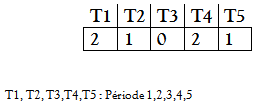
\includegraphics[scale=.5]{img/adopt_gene_repr.png}
			\caption{Représentation génétique adoptée}
			\label{fig:adopt_gene_repr}
		\end{center}
 \end{figure}
 \end{frame}
 
 \begin{frame}
 \frametitle{Aspects généraux aux deux méthodes de recherche proposées}
 \framesubtitle{Initialisation I}
	
	\begin{figure}[!h]
		\begin{center}
			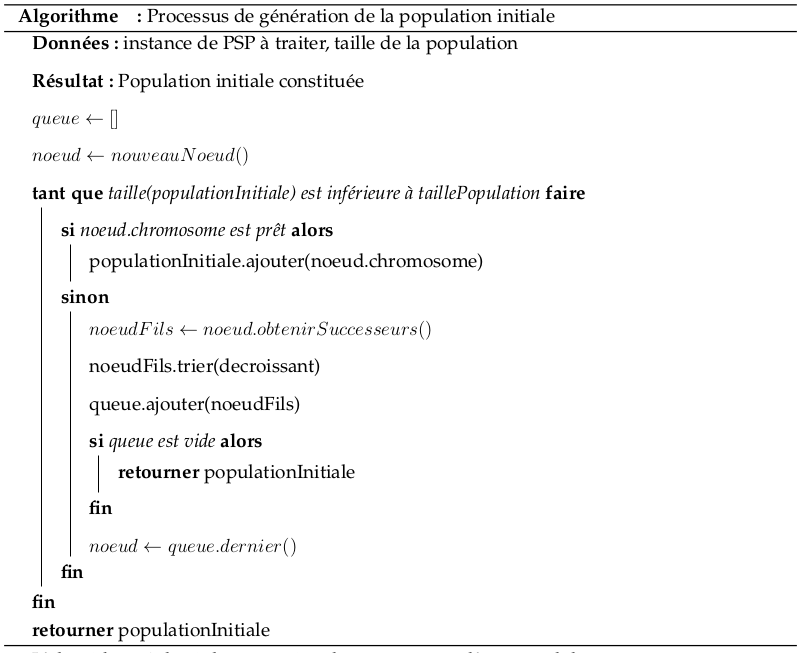
\includegraphics[scale=.4]{img/init_algo.png}
			%\caption{}
			\label{fig:adopt_gene_repr}
		\end{center}
 \end{figure}
	
 \end{frame}
 
 \begin{frame}
 \frametitle{Aspects généraux aux deux méthodes de recherche proposées}
 \framesubtitle{Initialisation II}
	
	\begin{figure}[!h]
		\begin{center}
			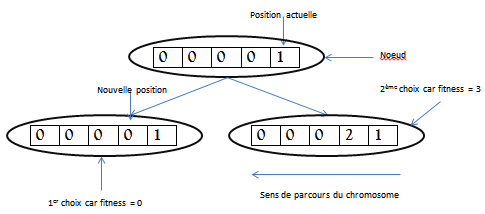
\includegraphics[scale=.5
			]{img/hill_climbing_fig.png}
			\caption{Schéma illustratif de l'application de l'algorithme du Hill climbing à une instance de PSP}
			%\label{fig:adopt_gene_repr}
		\end{center}
 \end{figure}
	
 \end{frame}
 
 \begin{frame}
 \frametitle{Aspects généraux aux deux méthodes de recherche proposées}
 \framesubtitle{Opérateurs génétiques I}
	
	\textbf{Sélection}
	\begin{figure}[!h]
		\begin{center}
			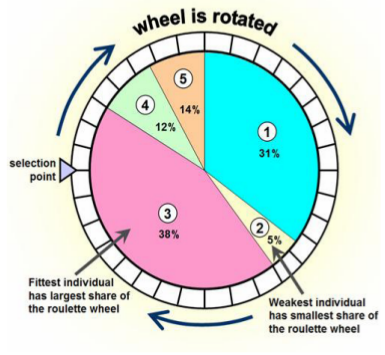
\includegraphics[scale=.5
			]{img/wheel_fig.png}
			\caption{Schéma illustratif de la méthode de \emph{roulette wheel}}
			%\label{fig:adopt_gene_repr}
		\end{center}
 \end{figure}
	
 \end{frame}
 
 \begin{frame}
 \frametitle{Aspects généraux aux deux méthodes de recherche proposées}
 \framesubtitle{Opérateurs génétiques II}
	
	\textbf{Croisement}
	\begin{figure}[!h]
		\begin{center}
			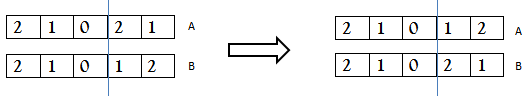
\includegraphics[scale=.5
			]{img/cross_over_fig.png}
			\caption{Schéma illustratif de la méthode de croisement utilisée}
			%\label{fig:adopt_gene_repr}
		\end{center}
 \end{figure}
	
 \end{frame}
 
 \begin{frame}
 \frametitle{Aspects généraux aux deux méthodes de recherche proposées}
 \framesubtitle{Opérateurs génétiques III}
	
	\textbf{Mutation}
	\begin{figure}[!h]
		\begin{center}
			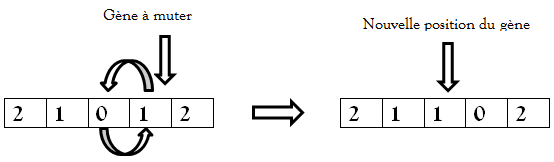
\includegraphics[scale=.5
			]{img/mutation_fig.png}
			\caption{Schéma illustratif de la méthode de mutation utilisée}
			%\label{fig:adopt_gene_repr}
		\end{center}
 \end{figure}
	
 \end{frame}
 
 \begin{frame}
 \frametitle{Aspects généraux aux deux méthodes de recherche proposées}
 \framesubtitle{Evaluation}
	
	%\textbf{}
	\begin{figure}[!h]
		\begin{center}
			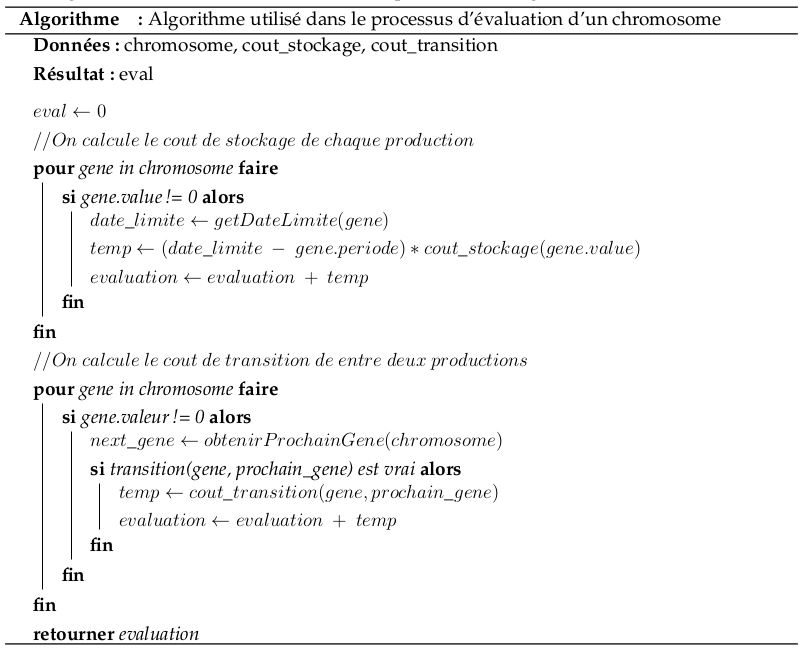
\includegraphics[scale=.4
			]{img/eval_algo.png}
			%\caption{Schéma illustratif de la méthode de mutation utilisée}
			%\label{fig:adopt_gene_repr}
		\end{center}
 \end{figure}
	
 \end{frame}
 
 \begin{frame}
 \frametitle{Aspects généraux aux deux méthodes de recherche proposées}
 \framesubtitle{Terminaison}
	
	\textbf{Deux critères de terminaison}
	\begin{itemize}
		\item Convergence de la population sur une solution;
		\item Absence de meilleures solutions à partir de celle trouvée.
	\end{itemize}
	
 \end{frame}
 
 \begin{frame}
 \frametitle{Aspects généraux aux deux méthodes de recherche proposées}
 \framesubtitle{Fonction de faisabilité}
	
	\begin{figure}[!h]
		\begin{center}
			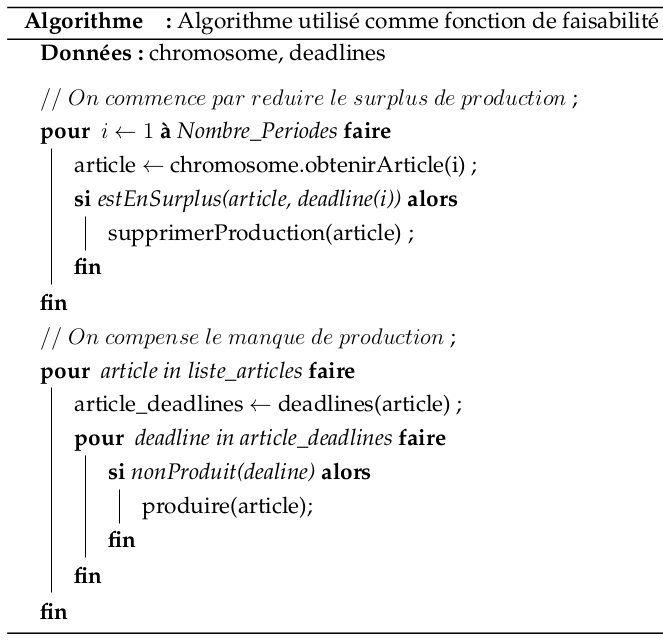
\includegraphics[scale=.4
			]{img/faisabilite_algo.png}
			%\caption{Schéma illustratif de la méthode de mutation utilisée}
			%\label{fig:adopt_gene_repr}
		\end{center}
 \end{figure}
	
 \end{frame}
 
 
 
 \subsection{Méthodes de recherche proposées}
 
 \begin{frame}
 \frametitle{Méthodes de recherche proposées}
 \framesubtitle{Algorithmes génétiques parallèles et hiérarchiques coarse-grained et
master-slave}
	
	Problématiques :
	\begin{itemize}
		\item Fréquence de migration;
		\item Choix et nombre de migrants;
		\item Topologie de connexions;
		\item Méthode d’intégration des migrants;
	\end{itemize}
	
 \end{frame}
 
 \begin{frame}
 \frametitle{Méthodes de recherche proposées}
 \framesubtitle{Algorithmes génétiques parallèles et hiérarchiques coarse-grained et
fine-grained}
	
	Problématiques :
	\begin{itemize}
		\item Fréquence de migration;
		\item Choix et nombre de migrants;
		\item Topologie de connexions;
		\item Méthode d’intégration des migrants;
	\end{itemize}
	
 \end{frame}
 
 \begin{frame}
 \frametitle{Méthodes de recherche proposées}
 \framesubtitle{Autres algorithmes implémentés I}
	
	\begin{itemize}
		\item Hybridation
		\begin{figure}[!h]
		\begin{center}
			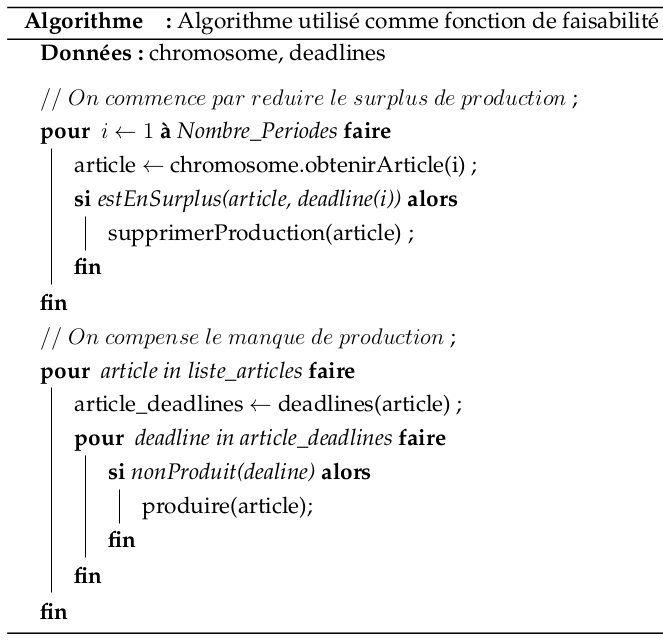
\includegraphics[scale=.3
			]{img/faisabilite_algo.png}
			%\caption{Schéma illustratif de la méthode de mutation utilisée}
			%\label{fig:adopt_gene_repr}
		\end{center}
 \end{figure}
	\end{itemize}
	
 \end{frame}
 
 \begin{frame}
 \frametitle{Méthodes de recherche proposées}
 \framesubtitle{Autres algorithmes implémentés II}
	
	\begin{itemize}
		\item Table de hash
		\begin{figure}[!h]
		\begin{center}
			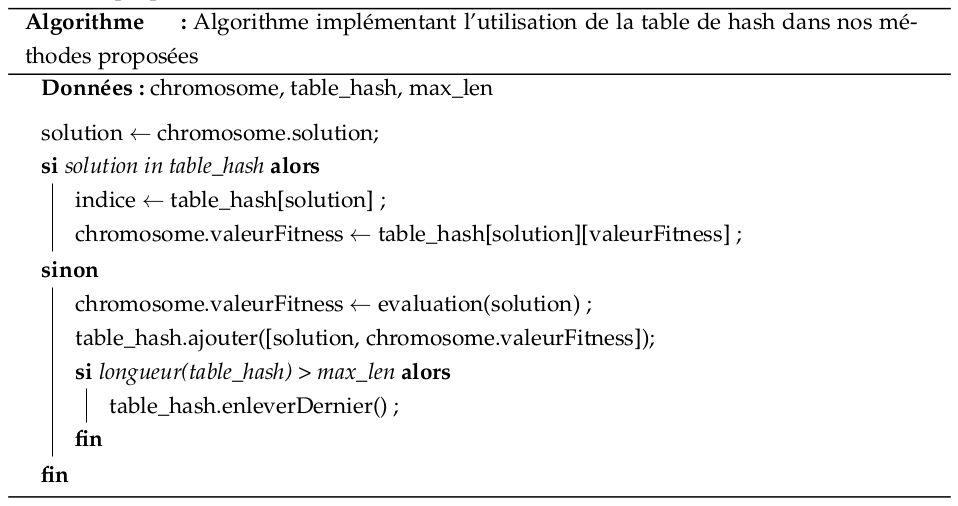
\includegraphics[scale=.4
			]{img/hash_table_algo.png}
			%\caption{Schéma illustratif de la méthode de mutation utilisée}
			%\label{fig:adopt_gene_repr}
		\end{center}
 \end{figure}
	\end{itemize}
	
 \end{frame}
 
 
 
 % Résultats et discussion
 \section{Résultats et discussion}
 \subsection{Données et paramètres de test}
 \begin{frame}
 \frametitle{Résultats et discussion}
 \framesubtitle{Données et paramètres de test}
 \begin{itemize}
					\item[-] Taille de la population : 25 individus par processus ;
			        \item[-] Probabilité de mutation : 5\%;
			        \item[-] Probabilité de croisement : 80\%;
			        \item[-] Nombre de migrants : 1 individu;
		 	        \item[-] Nombre de processus esclaves : 2 processus;
			        \item[-] Nombre de processus principaux : 2 processus;
			        \item[-] Nombre de générations avant migration : 0 génération (la migration intervient après une convergence).
				\end{itemize}
 \end{frame}
 
 \subsection{Résultats expérimentaux des algorithmes génétiques parallèles hiérarchiques fine-grained et coarse-grained}
 
 \begin{frame}
 \frametitle{Résultats expérimentaux des algorithmes génétiques parallèles hiérarchiques fine-grained et coarse-grained}
 \framesubtitle{HFC-PGA et CP}
 \begin{figure}[!h]
		\begin{center}
			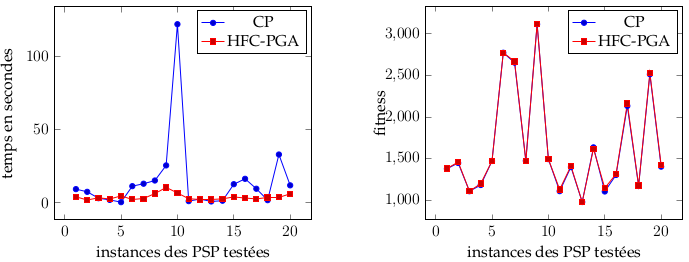
\includegraphics[scale=.4
			]{img/cp_hfc.png}
			%\caption{Schéma illustratif de la méthode de mutation utilisée}
			%\label{fig:adopt_gene_repr}
		\end{center}
 \end{figure}
 \end{frame}
 
 \begin{frame}
 \frametitle{Résultats expérimentaux des algorithmes génétiques parallèles hiérarchiques fine-grained et coarse-grained}
 \framesubtitle{HFC-PGA et SA}
 \begin{figure}[!h]
		\begin{center}
			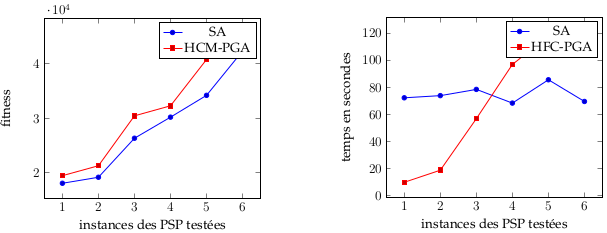
\includegraphics[scale=.4
			]{img/sa_hfc.png}
			%\caption{Schéma illustratif de la méthode de mutation utilisée}
			%\label{fig:adopt_gene_repr}
		\end{center}
 \end{figure}
 \end{frame}
 
 \subsection{Résultats expérimentaux des algorithmes génétiques parallèles hiérarchiques master-slave et coarse-grained}
 
 \begin{frame}
 \frametitle{Résultats expérimentaux des algorithmes génétiques parallèles hiérarchiques master-slave et coarse-grained}
 \framesubtitle{HCM-PGA et CP}
 \begin{figure}[!h]
		\begin{center}
			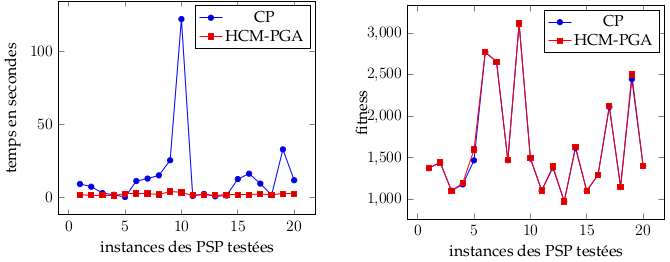
\includegraphics[scale=.4
			]{img/cp_hcm.png}
			%\caption{Schéma illustratif de la méthode de mutation utilisée}
			%\label{fig:adopt_gene_repr}
		\end{center}
 \end{figure}
 \end{frame}
 
 \begin{frame}
 \frametitle{Résultats expérimentaux des algorithmes génétiques parallèles hiérarchiques master-slave et coarse-grained}
 \framesubtitle{HCM-PGA et SA}
 \begin{figure}[!h]
		\begin{center}
			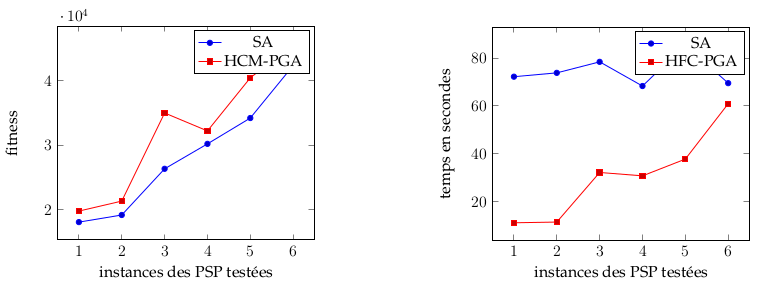
\includegraphics[scale=.4
			]{img/sa_hcm.png}
			%\caption{Schéma illustratif de la méthode de mutation utilisée}
			%\label{fig:adopt_gene_repr}
		\end{center}
 \end{figure}
 \end{frame}

 \subsection{Discussion} 
 
 % Conclusion
 \section*{Conclusion}
 \begin{frame}
  \frametitle{Conclusion}
 	\begin{center}
 		\LARGE{\texttt{Conclusion}}
 	\end{center}
 \end{frame}
 
 \begin{frame}
 	\begin{center}
 		\LARGE{\texttt{Merci pour votre attention}}
 	\end{center}
 \end{frame}
 
% \begin{frame}{•}
% 
% \end{frame}
 
 \end{document}